\chapter{Introduction}

There have been efforts to decarbonise the energy system in line with the targets outlined in the Paris Agreement at various administrative levels worldwide, ranging from political unions such and individual countries, to states, cities, local authorities, and even communities. Offshore wind energy, which only contributed 2,000 MW of renewable electricity in early 2010 \autocite{esteban2011}, has seen major developments since, with the United Kingdom (UK) alone installing 1,764 MW of new offshore wind generators in 2019 \autocite{windeurope2020}.

The \gls{smp} was published by the Scottish Government in October 2020, in line with their offshore wind policy statement commitments to reach a zero emission target by 2050 \autocite{govscot-smp}. This plan details 15 potential Plan Options, or development sites, in Scottish waters for commercial-scale offshore wind farm development, derived through an iterative process involving spatial planning and stakeholder engagement. Once these sites are identified, Crown Estate Scotland starts a seabed leasing round, where developers can apply to receive approval for constructing new commercial-scale offshore wind farms in Scotland \autocite{crownestate}.

The smallest of these sites, referred to as ``N4'', is in the northern region of Scotland and has a total area of 200 km\textsuperscript{2} and a maximum generating capacity potential of 1 GW (assuming a density of 5 MW/km\textsuperscript{2}), of which 100 \% development is deemed realistic. As shown in \autoref{fig:n4}, this site is adjacent to the northern coast of the Isle of Lewis in the Outer Hebrides (also known as the Western Isles or \textit{Na h-Eileanan Siar} in Scottish Gaelic), and is significantly close to the northern shoreline of the island, measuring just 4.5 km from the nearest vertex \autocite{naturescot-smp}.

\begin{figure}
  \centering
  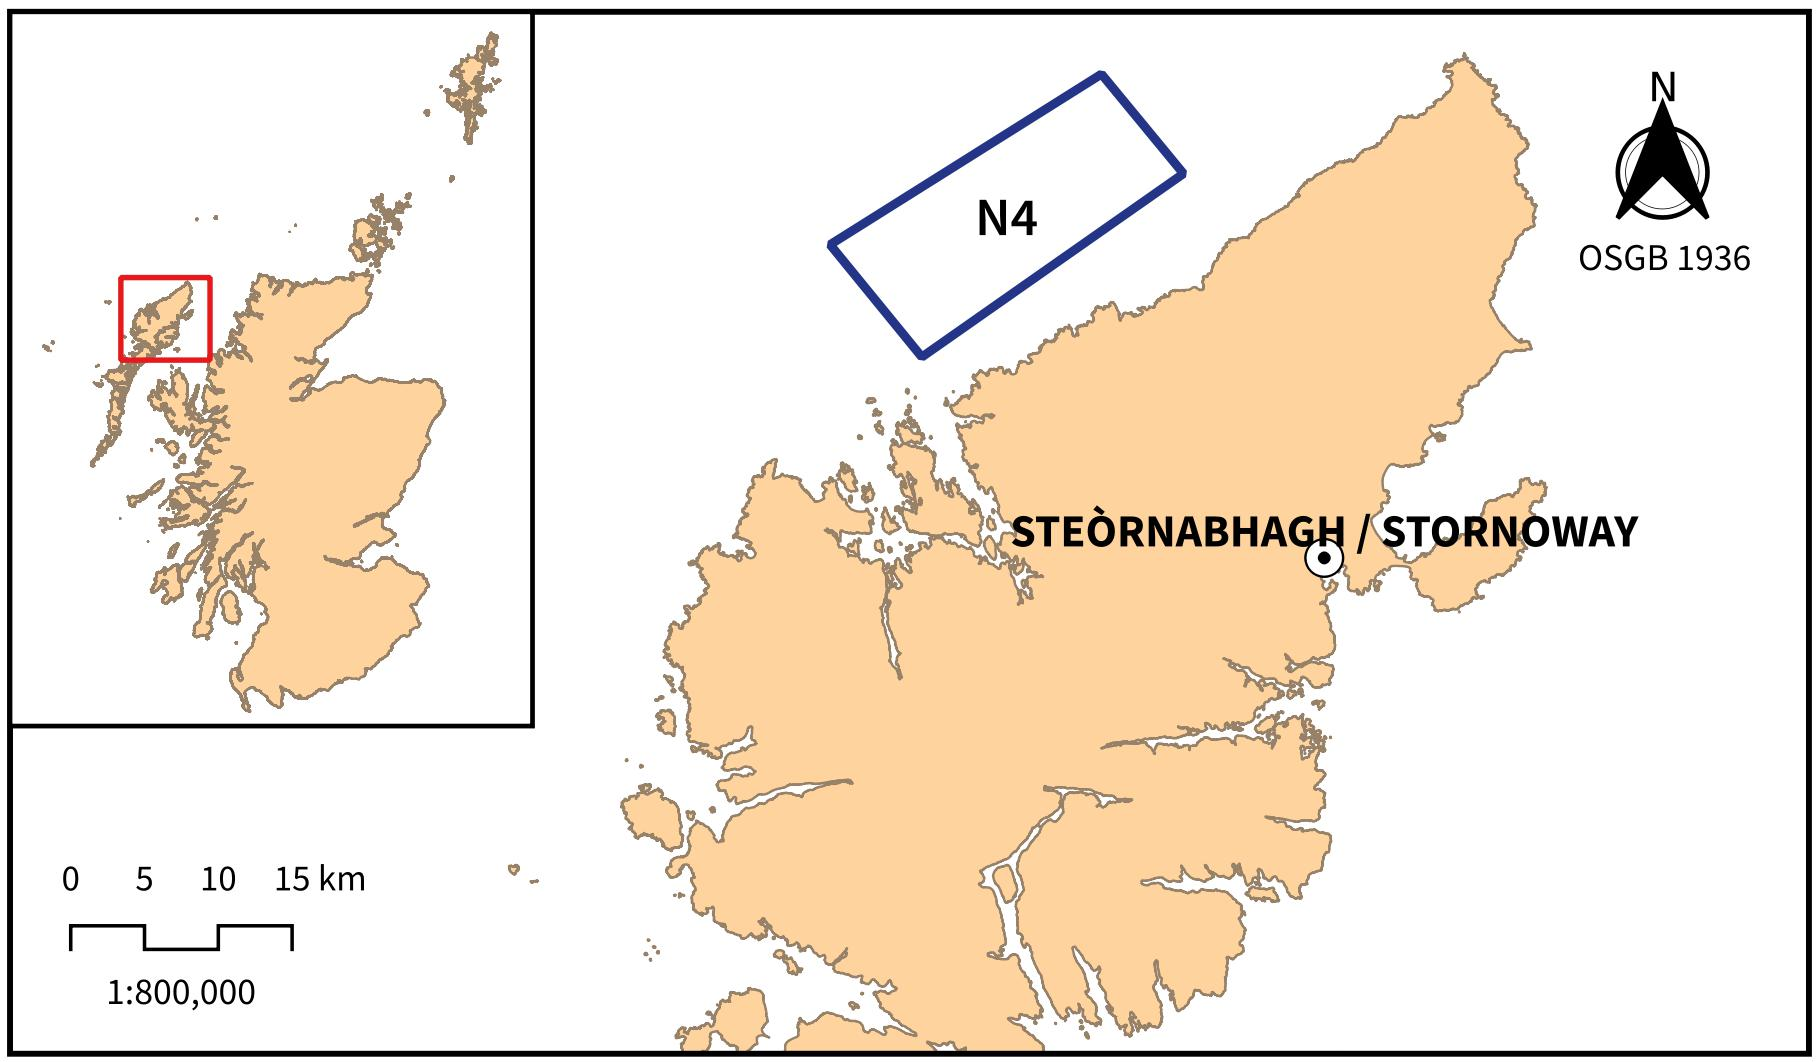
\includegraphics{images/maps/overview}
  \caption{A map showing the location of Sectoral Marine Plan Option N4 within the Isle of Lewis. The location of the Isle of Lewis within Scotland is shown in the inset. \label{fig:n4}}
\end{figure}

Based on responses to the draft \gls{smp} Plan Options by individuals and organisations \autocite{govscot-smpresponses}, there has been widespread opposition of Draft Plan Option SW1 (south-west region; outer Solway Firth), with over 300 negative responses \autocite{govscot-smp} from community members, local businesses, and fishers citing adverse impacts to the landscape, seascape, and socio-economic activities. As a result, SW1 was dropped from the final Plan Option. In contrast, there were very few responses pertaining to site N4, which indicates that Isle of Lewis communities have been generally unaware of the proposed site at the time of the government survey.

According to Comhairle nan Eilean Siar (the Outer Hebrides local government council) Local Development Plan, the Outer Hebrides is home to many cultural heritage and nature conservation sites, as well as communities that rely on tourism and small-scale economic activities \autocite{cnes-ldp}. Housing in the Outer Hebrides is predominantly through crofting tenure, i.e. ``a land tenure system of small scale food producers unique to the Scottish Highlands and Islands'' \autocite{crofting}, with high levels of community land ownership \autocite{cnes-ldp}. Despite this, Historic Environment Scotland neither supports nor opposes development at site N4, although they noted that adverse impacts are affected due to proximity to the shore, and mitigating these impacts is expected to be challenging \autocite{govscot-smpresponses}.

Considering the inshore location of site N4, developing the site into a commercial-scale offshore wind farm is expected to have adverse effects on the island communities. Therefore, it is crucial to quantify and analyse the potential impacts of this development on the island's landscape and industries. The results of this analysis can be used to increase awareness and understanding of these impacts in communities, helping them make informed decisions and participate effectively in future stakeholder meetings.

\section{Aims and objectives}

The aim of this project is to utilise geospatial methodologies to assess the impacts of commercial-scale offshore wind development at site N4, which is situated in the northern coastline of the Isle of Lewis in the Outer Hebrides.

\noindent The objectives of this project are to:

\begin{itemize}[noitemsep]
  \item generate a number of hypothetical commercial-scale offshore wind farm development scenarios to investigate the visual effects of varying the number and height of turbines installed;
  \item perform a viewshed analysis for each development scenario and compare the visual impacts in a number of identified viewpoints in the study area;
  \item identify environmental and socio-economic community impact assessment criteria and assess the suitability of site N4 using \gls{mca};
  \item conduct a participatory \gls{gis} session with community landowners affected by potential development at site N4 to gain their local knowledge and opinions; and
  \pagebreak
  \item propose an accessible method using \gls{gis} to improve public participation, understanding, and awareness of such large-scale projects.
\end{itemize}
